Machine learning is the study of algorithms and statistical models employed by computing systems
capable of performing tasks without explicit instruction. While traditional algorithms
rely on some specified input and a ruleset for determining the output, machine learning
is instead concerned with a set of generic algorithms which can find patterns
in a broad class of data sets. This section will give a brief overview of machine learning,
and more specifically the class of algorithms known as neural networks, and will follow closely the review by
% cite here
[Mehta et. al.] which the reader is encouraged to seek out.
\par
Examples of machine learning problems include identifying objects in images,
transcribing text from audio and making film recommendations to viewers based on their watch history.
Machine learning problems are often subdivided into estimation and prediction problems.
In both cases, we choose some observable $\bm{x}$ (e.g. the period of a pendulum)
related to some parameters $\bm{\theta}$ (e.g. the length and the gravitational constant)
through a model $p(\bm{x} \lvert \bm{\theta})$ that describes the probability of observing
$\bm{x}$ given $\bm{\theta}$. Subsequently we perform an experiment to obtain a dataset
$\bm{X}$ and use these data to fit the model. Fitting the model means finding
the parameters $\hat{\bm{\theta}}$ that provide the best explanation for the data. 
\textit{Estimation} problems are concerned with the accuracy of $\hat{\bm{\theta}}$, whereas
prediction problems are concerned with the ability of the model $p(\bm{x} \lvert \bm{\theta})$
to make new predictions.
Physics has traditionally been more concerned with the estimation of model parameters, while in
this thesis we will be focused on the accuracy of the model.
\par
Many problems in machine learning are defined by the same set of ingredients.
The first is the dataset $\mathcal{D} = (\bm{X}, \bm{Y})$, where $\bm{X}$ is a matrix
containing observations of the independent variables $\bm{x}$, and $\bm{Y}$ is a matrix containing
observations of dependent variables. Second is a model $\bm{F}: \bm{x} \rightarrow \bm{y}$
which is a function of the parameters $\bm{\theta}$. Finally we have a cost function
$\mathcal{C}\left(\bm{Y}, \bm{F}\left(\bm{X} ; \bm{\theta}\right)\right)$
that judges the performance of our model at generating predictions.
\newline
In the case of linear regression we consider a set of independent observations
$ \bm{X} = 
\begin{bmatrix}
\bm{x}_1 & \bm{x}_2 & \dots & \bm{x}_N
\end{bmatrix}
$
related to a set of dependent observations $\bm{y} = (y_1, y_2, \dots,y_N)$
through a linear model 
%\newline
$f(\bm{x} ; \bm{\theta}) = 
x_1\cdot w_1 + x_2\cdot w_2 + \dots + x_P\cdot w_P$,
with parameters $\bm{\theta} = (w_1, w_2, \dots,w_P)$. The cost function
is the well known sum of least squares $\mathcal{C}(\bm{y}, f(\bm{X} ; \bm{\theta}))
= \sum_i^N (y_i - f(\bm{x}_i ; \bm{\theta}))^2 $ and the best fit is chosen as the set
of parameters which minimize this cost function: $\hat{\bm{\theta}} = \underset{\bm{\theta}}
{\text{argmin}} \ \mathcal{C}(\bm{Y}, f(\bm{X} ; \bm{\theta})) $.

\subsection{Basics of statistical learning}
% needs revision
Statistical learning theory is a field of statistics dealing with the problem
of making predictions from data. We begin with an unknown function \newline
$y = f(x)$ and our goal is to develop a function $h(x)$
such that $h \sim f$. We fix a hypothesis set $\mathcal{H}$ that the
algorithm is willing to consider. The expected error of a particular $h$
over all possible inputs $x$ and outputs $y$ is:
$$ E[h] = \int_{X \times Y} \mathcal{C}(h(x), y) \rho(x,y) dx dy ,$$
where $\mathcal{C}$ is a cost function and $\rho(x,y)$ is the joint probability
distribution for $x$ and $y$. This is known as the \textit{expected error}.
Since this is impossible to compute without knowledge of the probability distribution
$\rho$, we instead turn to the \textit{empirical error}. Given $n$ data points
the empirical error is given as:
$$ E_S[h] = \frac{1}{n} \sum_i^n \mathcal{C}(h(x_i), y_i) .$$
The \textit{generalization error} is defined as the difference
between the expected and empirical errors:
$$ G = E[h] - E_S[h] .$$
We say an algorithm is able to learn from data or \textit{generalize} if 
$$ \lim_{n\to\infty} G = 0 .$$

We are in general unable to compute the expected error, and therefore unable
to compute the generalization error. The most common approach known as
\textit{cross-validation} is to estimate the
generalization error by subdividing our dataset into a \textit{training} set
and a \textit{test} set. The value of the cost function on the training set
is called the \textit{in-sample} error and the value of the cost
function on the test set the \textit{out-of-sample} error.
Assuming the dataset is sufficiently large and representative of $f$, and the subsampling
into train and test datasets is unbiased, the in-sample error
can serve as an appropriate proxy for the generalization error.
\newline
In figure \ref{fig:in-out}
we show the typical evolution of the errors as the number of data points increase.
It is assumed that the function being learned is sufficiently complicated
that we cannot learn it exactly, and that we have a sizeable number of data points
available. The in-sample error will decrease monotonically, as our model
is not able to learn the underlying data exactly. In contrast, the out-of-sample
error will decrease, as the sampling noise decreases and the training
data set becomes more representative of the underlying probability distribution.
In the limit, these errors both approach same value, which is known the model
\textit{bias}. The bias represents the best our model could do in the infinite data limit.
The out-of-sample error produced from the sampling noise
is known as \textit{variance}, and will vanish completely
given an infinite representative data set.

% create own figures or cite properly
\begin{figure}
    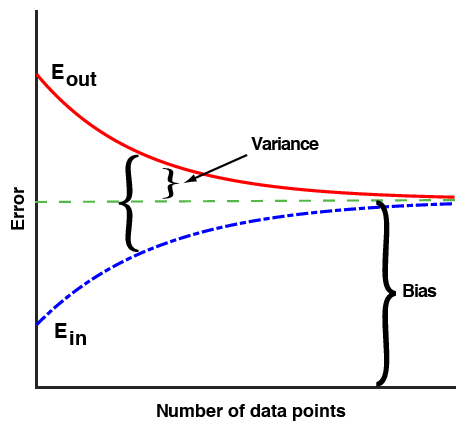
\includegraphics[width=\linewidth]{in-out-sample.png}
    \caption{Typical in-sample and out-of-sample error as a function
    of the number of data points. It is assumed that the number
    of data points is not small, and that the true function
    cannot be exactly fit.}
\end{figure}

In figure \ref{fig:bias-variance} we show the typical evolution
of the out-of-sample error as the model \textit{complexity} increases.
Model complexity is a measure of the degrees of freedom in the model space,
for example the number of coefficients in a polynomial regression.
In the figure we can see that bias decreases monotonically as model complexity
increases, as the model is able to fit a larger space of functions.
However, the variance will also increase as the model becomes more
susceptible to sampling noise. In general the lowest out-of-sample error,
and therefore generalization error, is achieved at an intermediate
model complexity. We also find that as model complexity increases,
a larger amount of data points is required to be able to reasonably
fit the true function.

% create own figures or cite properly
\begin{figure}
    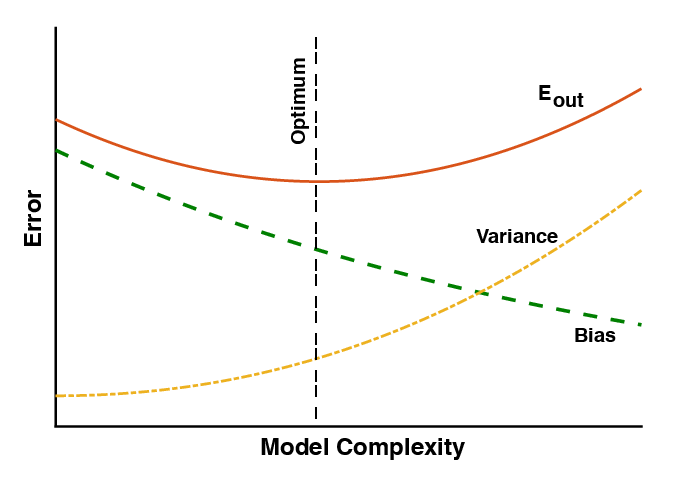
\includegraphics[width=\linewidth]{bias-variance.png}
    \caption{Typical out-of-sample error as a function
    of model complexity for a fixed dataset. Bias decreases monotonically with
    model complexity, while variance increases as a result of
    sampling noise.}
\end{figure}

\subsection{Bias-variance decomposition}
Consider a dataset $\mathcal{D}(\bm{X}, \bm{y})$ of $n$ pairs
of independent and dependent variables. Assume the true data
is generated from a noisy model:
$$ y = f(\bm{x}) + \epsilon ,$$
where $\epsilon$ is normally distributed with mean $\mu$ and
standard deviation $\sigma$. Assume that we have an estimator $h(\bm{x}; \bm{\theta})$
trained by minimizing a cost function $\mathcal{C}(\bm{y}, h(\bm{x}))$
which we take to be the sum of squared errors:
$$ \mathcal{C}(\bm{y}, h(\bm{x})) = \sum_i^n (y_i - h(\bm{x}_i; \bm{\theta}))^2 .$$
Our best estimate for the model parameters:
$$ \bm{\theta}_{\mathcal{D}} = \underset{\bm{\theta}}{\argmin} \
\mathcal{C}(\bm{y}, h(\bm{x}; \bm{\theta})) ,$$
is a function of the dataset $\mathcal{D}$. If we imagine we have a set of
datasets $\mathcal{D}_j = (\bm{y}_j, \bm{X}_j)$, each with $n$ samples, we would like to calculate
the expectation value of the cost function over all these datasets $E_{\mathcal{D}, \epsilon}$.
We would also like to calculate the expectation value over different instances of the noise $\epsilon$.
The expected generalization error can be decomposed as:
% more in depth?
\begin{equation}
\begin{split}
    E_{\mathcal{D}, \epsilon} [\mathcal{C}(\bm{y}, h(\bm{X} ; \bm{\theta}_{\mathcal{D}}))]
    &= E \left[ \sum_i (y_i - h(\bm{x}_i ; \bm{\theta}_{\mathcal{D}}))^2 \right] \\
    &= \sum_i \sigma_{\epsilon}^2 + E_{\mathcal{D}}[(f(\bm{x}_i) - f(\bm{x}_i ; \bm{\theta}_{\mathcal{D}}))^2] .
\end{split}
\end{equation}

The second term can be further decomposed as
\begin{equation}
\begin{split}
    &E_{\mathcal{D}}[(f(\bm{x}_i) - f(\bm{x}_i ; \bm{\theta}_{\mathcal{D}}))^2] \\
    &= (f(\bm{x}_i) - E_{\mathcal{D}}[h(\bm{x}_i ; \bm{\theta}_{\mathcal{D}})])^2
    + E[(h(\bm{x}_i ; \bm{\theta}_{\mathcal{D}}) - E[h(\bm{x}_i ; \bm{\theta}_{\mathcal{D}}])^2]
\end{split}
\end{equation}

The first term is what we have referred to as the bias:

\begin{equation}
    \text{Bias}^2 = \sum_i (f(\bm{x}_i) - E_{\mathcal{D}}[h(\bm{x}_i ; \bm{\theta}_{\mathcal{D}})])^2.
\end{equation}

The bias measures the expectation value of the deviation of our model from the true
function, i.e. the best we can do in the infinite data limit.
\newline
The second term is what we have referred to as the variance:
\begin{equation}
    \text{Var} = \sum_i  E[(h(\bm{x}_i ; \bm{\theta}_{\mathcal{D}}) - E[h(\bm{x}_i ; \bm{\theta}_{\mathcal{D}}])^2]
\end{equation}

The variance measures the deviation of our model due to finite-sampling effects.
Combining these effects we can decompose the out-of-sample error into:
\begin{equation}
    E_{\text{out}} = \text{Bias}^2 + \text{Var} + \text{Noise},
\end{equation}

with $\text{Noise} = \sum_i \sigma_{\epsilon}^2$.
\newline
In general it can be much more difficult to obtain sufficient good data
than to train a very complex model. Therefore it is often useful in practice
to use a less complex model with higher bias, because it is less susceptible
to finite-sampling effects.

\subsection{Neural networks}
Artificial Neural Networks (ANN) or Deep Neural Networks (DNN) are
supervised learning models vaguely inspired by biological neural networks.

% own figure or cite
\begin{figure}
    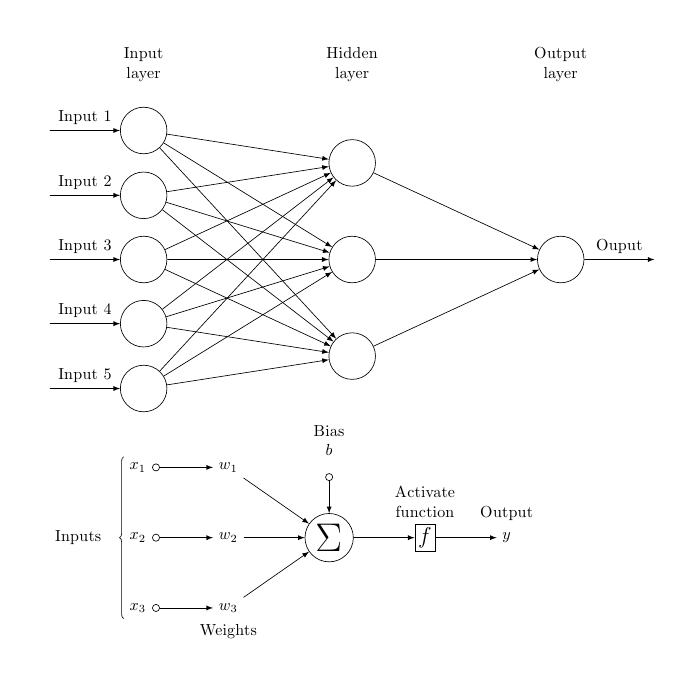
\includegraphics[width=\linewidth]{neural-networks.png}
    \caption{Text.}
\end{figure}

\subsection{Optimization}
More text.
